% ============================================================
% Reporte: Conversión de Decimal a Binario en Ensamblador x86
% Autor: Edson Joel Carrera Avila
% ============================================================

\documentclass[12pt, letterpaper]{article}

\usepackage[utf8]{inputenc}
\usepackage[T1]{fontenc}
\usepackage[english]{babel}
\usepackage{geometry}
\usepackage{graphicx}
\usepackage{listings}
\usepackage{xcolor}
\usepackage{booktabs}
\usepackage{amsmath}
\usepackage{hyperref}
\usepackage{fancyhdr}
\usepackage{float}
\usepackage{caption}
\usepackage{tikz}
\usetikzlibrary{shapes.geometric, arrows.meta, positioning}

\geometry{top=2.5cm, bottom=2.5cm, left=3cm, right=2.5cm}

% --- Colores y estilo de código ---
\definecolor{codegray}{rgb}{0.95,0.95,0.95}
\definecolor{codegreen}{rgb}{0.0,0.5,0.0}
\definecolor{codeblue}{rgb}{0.0,0.0,0.65}
\definecolor{codepurple}{rgb}{0.45,0.0,0.55}

\lstdefinelanguage{MASM}{
    morekeywords={PROC,ENDP,END,PUSH,POP,MOV,ADD,SUB,CALL,RET,JMP,
                  JE,JZ,JNZ,INC,DEC,CMP,TEST,BSR,SHL,SETC,LEA,
                  EXTERN,BYTE,DWORD,PTR,EBP,ESP,ESI,EDI,EAX,EBX,
                  ECX,EDX,AL,BL,CL,DL,.586,.model,.data,.code,
                  flat,stdcall,C,offset,option,casemap,none,
                  include,includelib,DUP},
    sensitive=false,
    morecomment=[l]{;}
}

\lstset{
    backgroundcolor=\color{codegray},
    basicstyle=\ttfamily\footnotesize,
    keywordstyle=\color{codeblue}\bfseries,
    commentstyle=\color{codegreen}\itshape,
    numbers=left, numberstyle=\tiny\color{gray}, numbersep=8pt,
    frame=single, rulecolor=\color{gray!50},
    breaklines=true, captionpos=b, tabsize=4,
    showstringspaces=false,
    literate=
        {á}{{\\'a}}1 {é}{{\\'e}}1 {í}{{\\'i}}1 {ó}{{\\'o}}1 {ú}{{\\'u}}1
        {Á}{{\\'A}}1 {É}{{\\'E}}1 {Í}{{\\'I}}1 {Ó}{{\\'O}}1 {Ú}{{\\'U}}1
        {ñ}{{\~n}}1 {Ñ}{{\~N}}1
}

% --- Encabezado ---
\pagestyle{fancy}
\fancyhf{}
\rhead{Práctica 04}
\lhead{\textit{Edson Joel Carrera Avila}}
\cfoot{\thepage}
\renewcommand{\headrulewidth}{0.5pt}

% ============================================================
\begin{document}

% --- Portada ---
\begin{titlepage}
    \centering
    \vspace*{1.5cm}

    {\Large \textbf{Universidad Autónoma de la Ciudad de México}}\\[0.3cm]
    {\large Licenciatura en Ingeniería de Software}\\[0.2cm]
    {\large Arquitectura de Computadoras}\\[2.5cm]

    \rule{\linewidth}{0.5pt}\\[0.4cm]
    {\LARGE \bfseries Práctica 04}\\[0.3cm]
    {\Large Conversión de Decimal a Binario en Ensamblador x86}\\[0.3cm]
    \rule{\linewidth}{0.5pt}\\[2cm]

    \begin{flushleft}
        \textbf{Alumno:} Edson Joel Carrera Avila \\[0.3cm]
        \textbf{Grupo:} 302 \\[0.3cm]
        \textbf{Profesor:} Prof. Mtro. Omar Nieto Crisóstomo \\[0.3cm]
        \textbf{Fecha:} \today
    \end{flushleft}
    \vfill
\end{titlepage}

\tableofcontents
\newpage

% ============================================================
\section{Introducción}

Esta práctica consiste en escribir un programa que combine \textbf{C++} y \textbf{lenguaje ensamblador x86}: C++ se encarga de la interacción con el usuario (leer el número y mostrar el resultado), mientras que una función escrita en ensamblador realiza la conversión del número decimal a su representación en binario, operando directamente sobre los bits del valor.

El objetivo principal no es simplemente ``convertir un número'', sino entender cómo el procesador manipula los datos en su forma más elemental, bit por bit. Para lograrlo, es necesario comprender dos conceptos fundamentales: la \textbf{representación binaria de los números} y las \textbf{operaciones de desplazamiento de bits}.

\subsection*{¿Qué es la representación binaria?}

Las computadoras almacenan y procesan todos sus datos en \textbf{sistema binario}: únicamente con los dígitos 0 y 1. Cada dígito binario se llama \textit{bit}. Un número entero de 32 bits es simplemente una secuencia de 32 ceros y unos, donde cada posición representa una potencia de 2:

\begin{equation}
    45_{10} = 1 \cdot 2^5 + 0 \cdot 2^4 + 1 \cdot 2^3 + 1 \cdot 2^2 + 0 \cdot 2^1 + 1 \cdot 2^0 = 101101_2
\end{equation}

\subsection*{¿Qué es un desplazamiento de bits (SHL)?}

La instrucción \texttt{SHL} (\textit{Shift Left}) mueve todos los bits de un registro un lugar hacia la izquierda. El bit que ``se cae'' por el extremo izquierdo no desaparece: el procesador lo atrapa en una bandera interna llamada \textbf{Carry Flag (CF)}, que puede leerse en el siguiente ciclo. Esta es la mecánica que permite extraer los bits de un número uno por uno, de mayor a menor.

% ============================================================
\section{Organización del programa}

El proyecto consta de dos archivos que trabajan en conjunto:

\begin{table}[H]
    \centering
    \begin{tabular}{@{}lp{9cm}@{}}
        \toprule
        \textbf{Archivo} & \textbf{Qué hace} \\
        \midrule
        \texttt{main.cpp}       & Pide al usuario un número decimal, llama a la función ensamblador y muestra el resultado binario en pantalla. \\
        \texttt{conversion.asm} & Recibe el número entero, localiza su bit más significativo, extrae cada bit de mayor a menor y construye la cadena de texto binaria en un buffer de memoria. \\
        \bottomrule
    \end{tabular}
    \caption{Archivos del proyecto}
\end{table}

El programa se divide internamente en cuatro fases:

\begin{itemize}
    \item \textbf{Preservar registros:} antes de usar \texttt{EBX} y \texttt{EDI}, sus valores se guardan en la pila para no interferir con C++.
    \item \textbf{Caso especial (cero):} si el número es 0, se escribe directamente \texttt{'0'} en el buffer y se termina.
    \item \textbf{Localizar el MSB:} la instrucción \texttt{BSR} encuentra la posición del bit más significativo; el número se alinea a la izquierda con \texttt{SHL} para preparar la extracción.
    \item \textbf{Ciclo de escritura:} en cada vuelta, \texttt{SHL} extrae un bit hacia la \textit{Carry Flag}; \texttt{SETC} lo lee y \texttt{ADD} lo convierte al carácter \texttt{'0'} o \texttt{'1'}.
\end{itemize}

El flujo general del programa es el siguiente:

\begin{figure}[H]
    \centering
    \resizebox{0.72\textwidth}{!}{%
        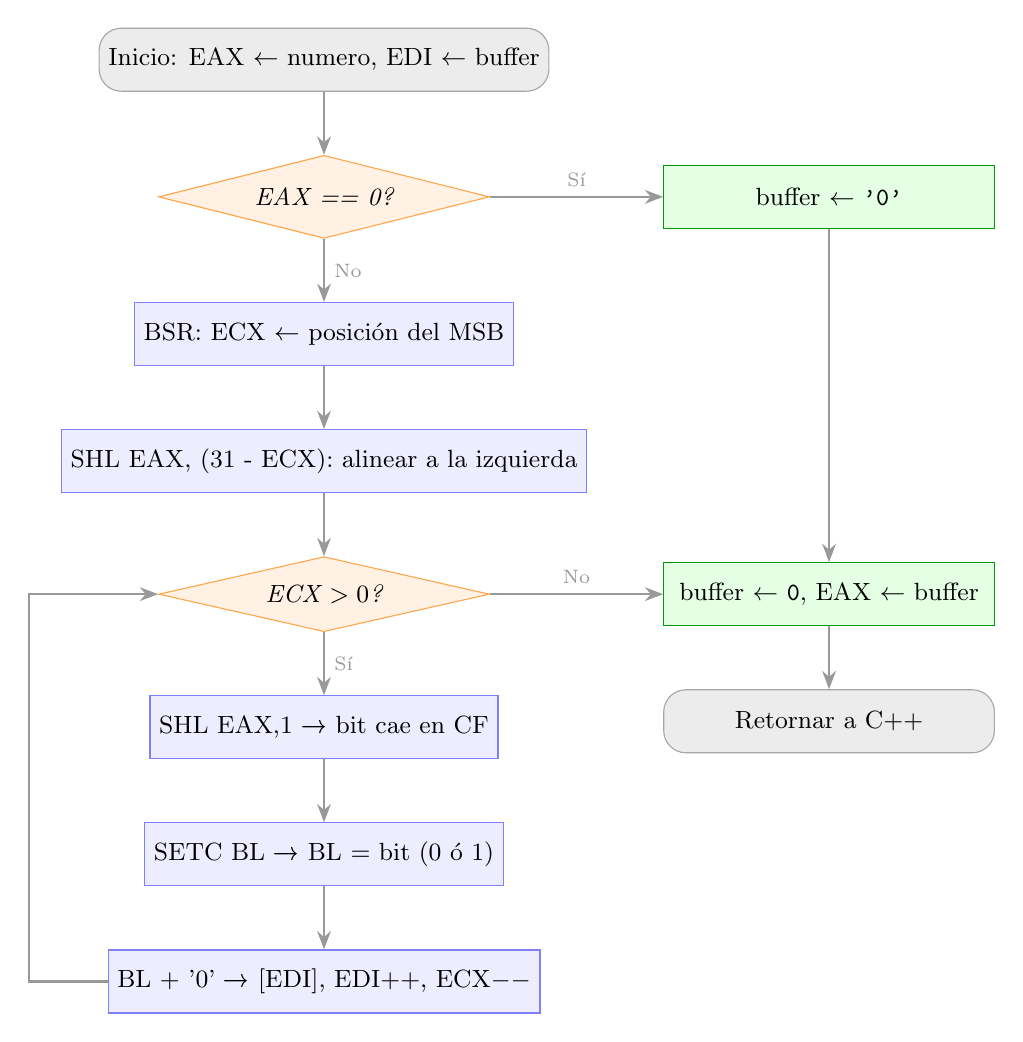
\begin{tikzpicture}[
            startstop/.style={rectangle, rounded corners=8pt, draw=gray!70, fill=gray!15,
                              minimum width=4.2cm, minimum height=0.8cm, font=\small},
            process/.style  ={rectangle, draw=blue!50, fill=blue!7,
                              minimum width=4.2cm, minimum height=0.8cm, font=\small},
            decision/.style ={diamond, aspect=2.4, draw=orange!70, fill=orange!10,
                              minimum width=4.2cm, font=\small\itshape, inner sep=1pt},
            result/.style   ={rectangle, draw=green!60!black, fill=green!10,
                              minimum width=4.2cm, minimum height=0.8cm, font=\small},
            arr/.style      ={-Stealth, thick, gray!80}
        ]
            % --- Nodos (Columna Principal y Bucle) ---
            \node[startstop] (inicio)  {Inicio: EAX $\leftarrow$ numero,\ EDI $\leftarrow$ buffer};
            \node[decision,  below=0.8cm of inicio]  (escero)  {EAX == 0?};
            \node[process,   below=0.8cm of escero]  (bsr)     {BSR: ECX $\leftarrow$ posición del MSB};
            \node[process,   below=0.8cm of bsr]     (alinear) {SHL EAX, (31 - ECX): alinear a la izquierda};
            \node[decision,  below=0.8cm of alinear] (loop)    {ECX $> 0$?};
            \node[process,   below=0.8cm of loop]    (extraer) {SHL EAX,1 → bit cae en CF};
            \node[process,   below=0.8cm of extraer] (setc)    {SETC BL → BL = bit (0 ó 1)};
            \node[process,   below=0.8cm of setc]    (escribir){BL + '0' → [EDI], EDI++, ECX$--$};

            % --- Nodos (Columna Derecha: Salidas y Fin) ---
            \node[result,    right=2.2cm of escero]  (cero)    {buffer $\leftarrow$ \texttt{'0'}};
            \node[result,    right=2.2cm of loop]    (fin)     {buffer $\leftarrow$ \texttt{0},\ EAX $\leftarrow$ buffer};
            \node[startstop, below=0.8cm of fin]     (ret)     {Retornar a C++};

            % --- Enlaces (Rutas directas sin cruces) ---
            \draw[arr] (inicio)  -- (escero);
            
            % Bifurcación Inicial (Caso EAX == 0)
            \draw[arr] (escero)  -- node[above, font=\scriptsize]{Sí} (cero);
            \draw[arr] (escero)  -- node[right, font=\scriptsize]{No} (bsr);
            
            % Preparación
            \draw[arr] (bsr)     -- (alinear);
            \draw[arr] (alinear) -- (loop);
            
            % Bifurcación del Bucle
            \draw[arr] (loop)    -- node[right, font=\scriptsize]{Sí} (extraer);
            \draw[arr] (loop)    -- node[above, font=\scriptsize]{No} (fin);
            
            % Interior del Bucle
            \draw[arr] (extraer) -- (setc);
            \draw[arr] (setc)    -- (escribir);
            
            % Línea de retorno del Bucle (viaja por el margen izquierdo vacío)
            \draw[arr] (escribir.west) -- ++(-1.0,0) |- (loop.west);
            
            % Unión hacia el retorno
            \draw[arr] (cero)    -- (fin);
            \draw[arr] (fin)     -- (ret);

        \end{tikzpicture}%
    }
    \caption{Diagrama de flujo del algoritmo de conversión decimal a binario}
\end{figure}

\begin{enumerate}
    \item C++ lee el número del usuario y llama a \texttt{decimalABinario} pasándolo como parámetro.
    \item El ensamblador verifica si el número es cero (caso especial).
    \item \texttt{BSR} localiza el bit más alto; \texttt{SHL} alinea el número para que ese bit quede en el extremo izquierdo de \texttt{EAX}.
    \item El ciclo extrae bit por bit con \texttt{SHL}: cada bit que ``se derrama'' por la izquierda es capturado por \texttt{SETC} y escrito como \texttt{'0'} o \texttt{'1'} en el buffer.
    \item Al terminar el ciclo, se coloca el terminador de cadena y se retorna la dirección del buffer a C++.
    \item C++ recibe el puntero e imprime la cadena resultante.
\end{enumerate}

% ============================================================
\section{Código fuente}

\subsection{Código C++ (main.cpp)}

\begin{lstlisting}[language=C++, caption={main.cpp --- Interfaz con el usuario}]
#include <iostream>
using namespace std;

extern "C" char* decimalABinario(int numero);

int main() {
    int decimal;

    cout << "Ingresa un numero decimal: ";
    cin >> decimal;

    char* binario = decimalABinario(decimal);

    cout << "DEC: " << decimal << endl;
    cout << "BIN: " << binario << endl;

    return 0;
}
\end{lstlisting}

\subsection{Código ensamblador (conversion.asm)}

\begin{lstlisting}[language=MASM, caption={conversion.asm --- Conversión de decimal a binario}]
.586
.model flat, C

.data
    buffer  BYTE  33 DUP(0)     ; 32 bits + terminador nulo

.code

decimalABinario PROC numero:DWORD

    push ebx                    ; Guardamos EBX en la pila
    push edi                    ; Guardamos EDI en la pila

    mov  eax, numero            ; EAX = numero a convertir
    lea  edi, buffer            ; EDI apunta al buffer de salida

    test eax, eax               ; ?El numero es cero?
    jz   caso_cero              ; Si es cero, caso especial

    bsr  ecx, eax               ; ECX = posicion del bit mas significativo

    mov  edx, 31
    sub  edx, ecx               ; EDX = cuantos lugares desplazar
    push ecx                    ; Guardamos ECX (SHL sobreescribira CL)
    mov  cl, dl                 ; CL = lugares a desplazar
    shl  eax, cl                ; Alineamos el MSB al extremo izquierdo
    pop  ecx                    ; Recuperamos el contador de bits
    inc  ecx                    ; +1 para incluir el MSB en el ciclo

escribir_bits:
    shl  eax, 1                 ; El bit mas alto cae a la Carry Flag
    setc bl                     ; BL = 1 si CF=1, BL = 0 si CF=0
    add  bl, '0'                ; Convertimos a caracter '0' o '1'
    mov  BYTE PTR [edi], bl     ; Escribimos en el buffer
    inc  edi                    ; Avanzamos el puntero
    dec  ecx                    ; Un bit menos
    jnz  escribir_bits          ; Repetir si quedan bits
    jmp  fin_funcion

caso_cero:
    mov  BYTE PTR [edi], '0'
    inc  edi

fin_funcion:
    mov  BYTE PTR [edi], 0      ; Terminador de cadena
    lea  eax, buffer            ; Retornamos la direccion del buffer
    pop  edi
    pop  ebx
    ret

decimalABinario ENDP

END
\end{lstlisting}

% ============================================================
\section{Instrucciones x86 utilizadas}

\begin{table}[H]
    \centering
    \begin{tabular}{@{}lp{9cm}@{}}
        \toprule
        \textbf{Instrucción} & \textbf{Qué hace en términos simples} \\
        \midrule
        \texttt{MOV}  & Copia un valor de un lugar a otro (entre registro y memoria). \\
        \texttt{LEA}  & Carga en un registro la \textit{dirección} de una variable, no su contenido. \\
        \texttt{TEST} & Compara un valor consigo mismo sin modificarlo; activa la bandera de cero si el resultado es 0. \\
        \texttt{JZ}   & Salta si la bandera de cero está activa (el valor comparado era 0). \\
        \texttt{JNZ}  & Salta si la bandera de cero \textit{no} está activa (el valor no era 0). \\
        \texttt{JMP}  & Salta incondicionalmente a otra parte del código. \\
        \texttt{BSR}  & Busca de derecha a izquierda el primer bit en 1 y guarda su posición. \\
        \texttt{SHL}  & Desplaza todos los bits hacia la izquierda; el bit que ``se cae'' queda en la \textit{Carry Flag}. \\
        \texttt{SETC} & Escribe 1 en un registro si la \textit{Carry Flag} está activa; escribe 0 si no. \\
        \texttt{ADD}  & Suma dos valores y guarda el resultado en el primero. \\
        \texttt{INC}  & Incrementa en 1 el valor del operando. \\
        \texttt{DEC}  & Decrementa en 1 el valor del operando. \\
        \texttt{PUSH} & Guarda un valor en la pila de memoria. \\
        \texttt{POP}  & Recupera el último valor guardado en la pila. \\
        \texttt{RET}  & Regresa el control al código que llamó a esta función. \\
        \bottomrule
    \end{tabular}
    \caption{Instrucciones x86 utilizadas en el programa}
\end{table}

% ============================================================
\section{El rol de los registros}

En este programa intervienen varios registros del procesador, cada uno con una responsabilidad específica:

\begin{itemize}
    \item \textbf{EAX} (\textit{Extended Accumulator Register}): contiene el número a convertir. A medida que el ciclo avanza, sus bits van siendo extraídos uno por uno mediante desplazamientos.
    \item \textbf{ECX} (\textit{Extended Counter Register}): actúa como contador del ciclo. Se inicializa con la cantidad de bits significativos del número y se decrementa en cada iteración.
    \item \textbf{EDX} (\textit{Extended Data Register}): almacena temporalmente la cantidad de lugares a desplazar para la alineación inicial del número.
    \item \textbf{EBX} / \textbf{BL}: \texttt{BL} (byte bajo de \texttt{EBX}) recibe el bit extraído vía \texttt{SETC} y lo convierte al carácter de texto correspondiente antes de escribirlo.
    \item \textbf{EDI} (\textit{Extended Destination Index}): actúa como puntero de escritura sobre el buffer. Avanza un byte en cada iteración.
    \item \textbf{CL}: byte bajo de \texttt{ECX}; es el único registro que \texttt{SHL} acepta como operando de desplazamiento variable.
\end{itemize}

La variable \texttt{buffer} se declara en \texttt{.data} con 33 bytes inicializados en 0: 32 para los dígitos binarios y 1 para el terminador de cadena que C++ necesita para saber dónde termina la cadena.

% ============================================================
\section{Ejemplo de ejecución}

Para el número decimal \textbf{45}:

\begin{table}[H]
    \centering
    \begin{tabular}{@{}ccccc@{}}
        \toprule
        \textbf{Iteración} & \textbf{Bit extraído (CF)} & \textbf{BL} & \textbf{Carácter escrito} & \textbf{ECX restante} \\
        \midrule
        1 & 1 & 1 & \texttt{'1'} & 5 \\
        2 & 0 & 0 & \texttt{'0'} & 4 \\
        3 & 1 & 1 & \texttt{'1'} & 3 \\
        4 & 1 & 1 & \texttt{'1'} & 2 \\
        5 & 0 & 0 & \texttt{'0'} & 1 \\
        6 & 1 & 1 & \texttt{'1'} & 0 \\
        \bottomrule
    \end{tabular}
    \caption{Extracción bit a bit de 45 = 101101\textsubscript{2}}
\end{table}

\begin{figure}[H]
    \centering
    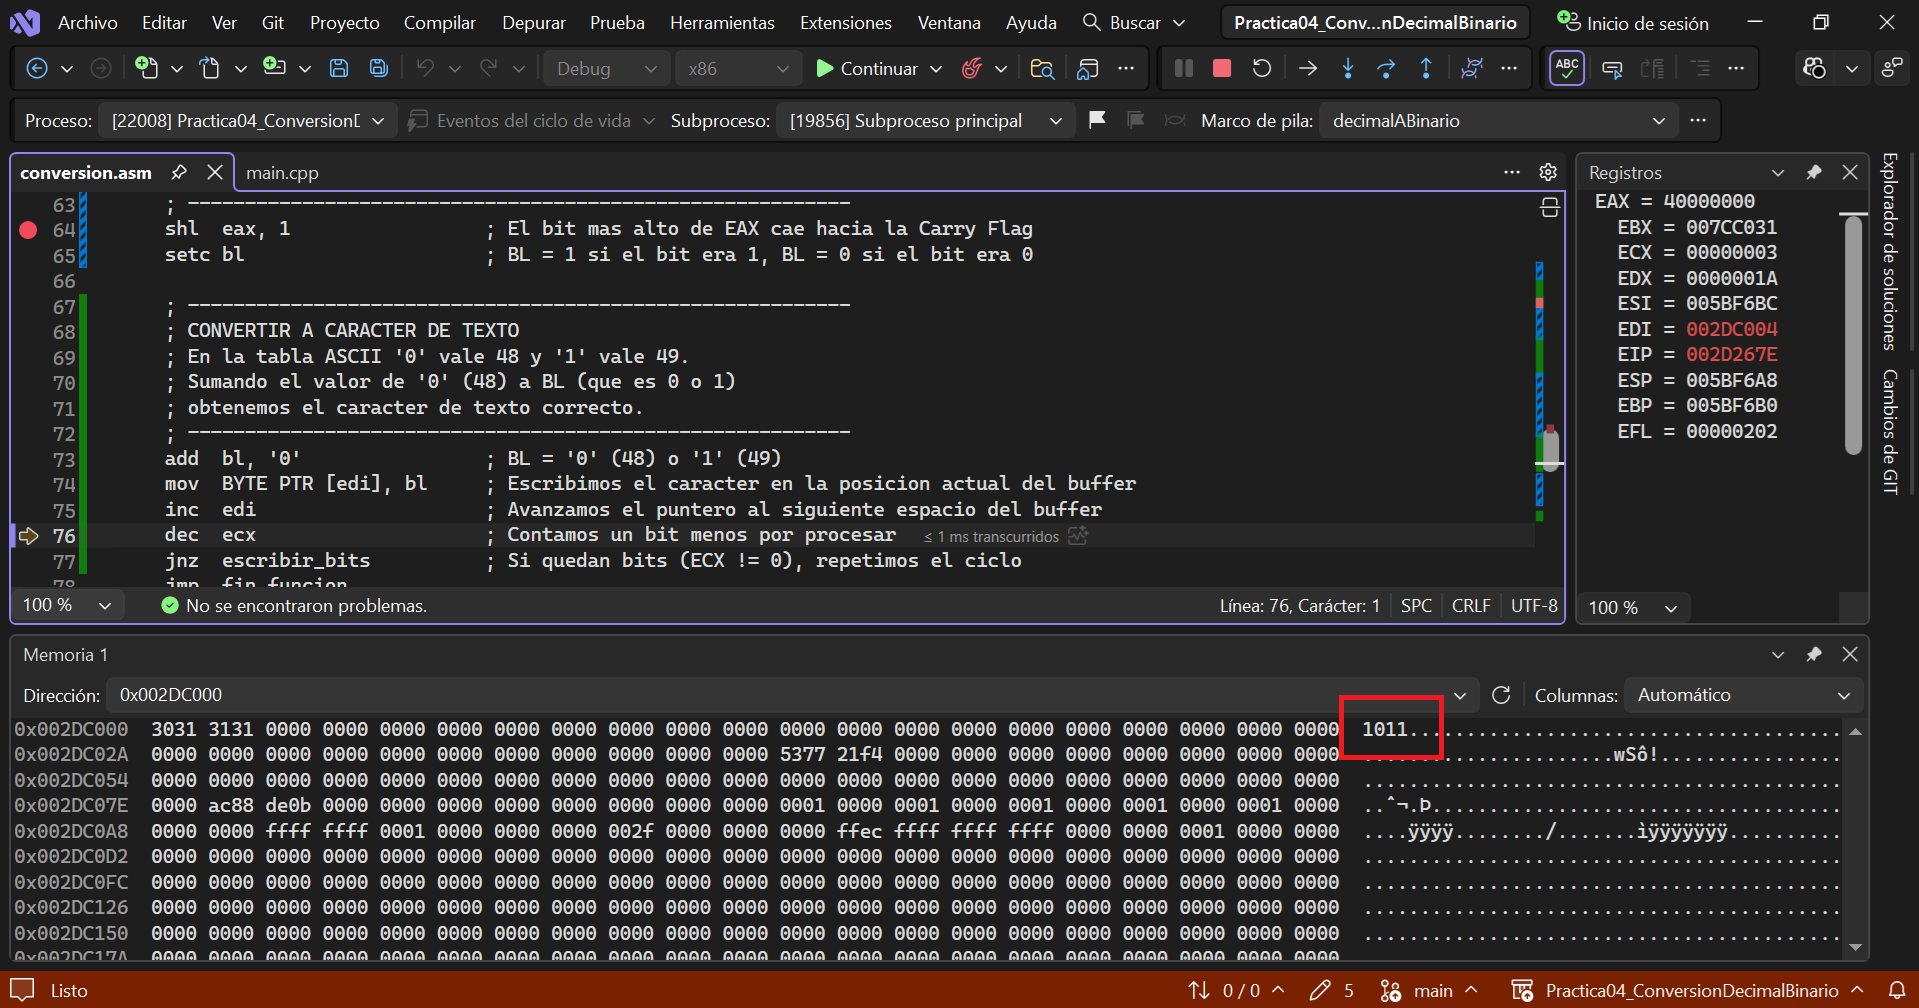
\includegraphics[width=1\textwidth]{memoria_buffer.png}
    \caption{Conversión de 45 DEC a BIN, donde buffer registra los cambios.}
    \label{fig:memoria_buffer}
\end{figure}

\begin{figure}[H]
    \centering
    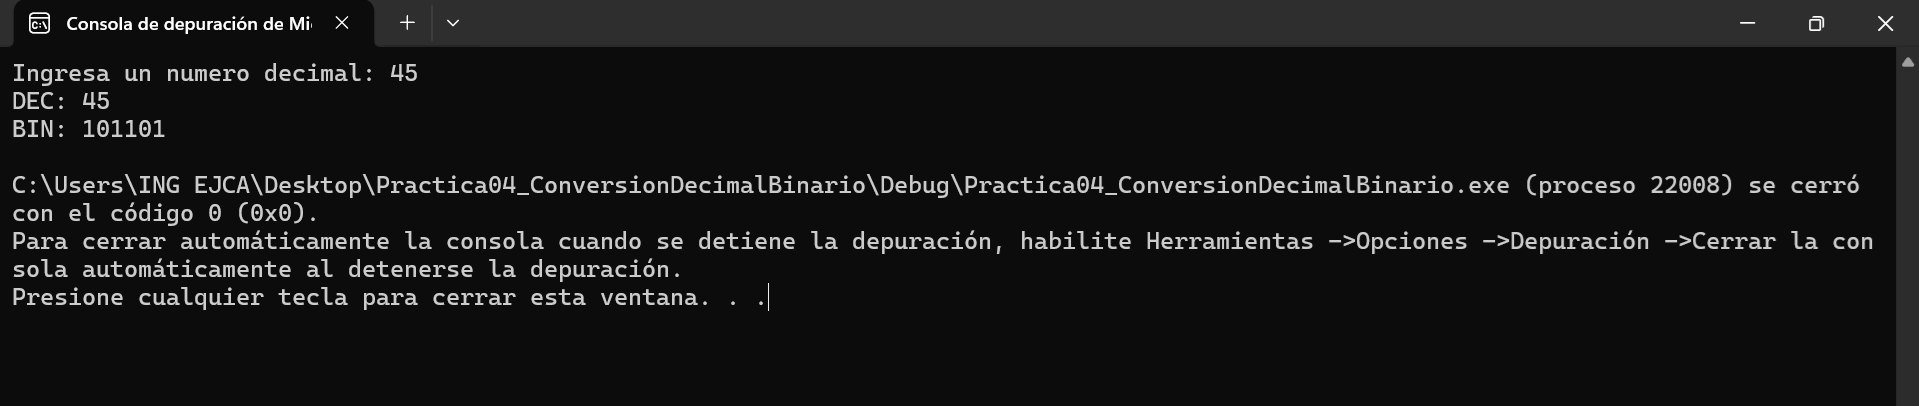
\includegraphics[width=1\textwidth]{consola_resultado.png}
    \caption{Salida en consola: DEC 45 → BIN 101101}
    \label{fig:consola_resultado}
\end{figure}

\section{Repositorio GitHub}

https://github.com/7mo-ArquitecturaComputadoras/Practica04\_ConversionDecimalBinario

% ============================================================
\section{Conclusiones}

\begin{itemize}
    \item El programa demuestra que \textbf{convertir a binario es leer los bits de un número uno por uno}: la computadora no ``calcula'' la representación binaria, simplemente expone los bits que ya estaban ahí desde el principio.
    \item La instrucción \texttt{BSR} permite encontrar el bit más significativo en un solo paso de hardware, evitando ceros innecesarios a la izquierda sin necesidad de un ciclo adicional.
    \item El uso combinado de \texttt{SHL} y \texttt{SETC} es un patrón idiomático en ensamblador para extraer bits de forma secuencial: cada desplazamiento a la izquierda ``derrama'' un bit hacia la \textit{Carry Flag}, donde puede leerse directamente.
    \item La \textbf{interfaz entre C++ y ensamblador} mediante \texttt{extern "C"} ilustra cómo los lenguajes de alto nivel pueden delegar operaciones críticas de bajo nivel a rutinas escritas directamente en ensamblador.
    \item Esta práctica evidencia que lo que un lenguaje como Python hace con \texttt{bin(45)} produce exactamente la misma secuencia de bits que este programa extrae manualmente: la diferencia es que aquí el proceso es completamente visible y controlado por el programador.
\end{itemize}

\end{document}
